\chapter{Choix technologiques}
    \section{Language C++}
        La première étape dans ce projet a été de choisir le language dans lequel il serait développé: la contrainte qui nous était imposée 
        était le choix entre le language C et ses dérivés.
        \\ Le C est un language de programmation généraliste et bas niveau\footnote{Près de la machine. En C beaucoup de résponsabilités sont laissées au développeur, comme l'allocation mémoire} inventé dans les années 1970. C'est un des language les plus utilisé 
        au monde, pionnier du monde informatique, qui a inspiré nombre d'autre language et donné naissance à des dérivés comme le C\#\footnote{Prononcer ``C sharp''}, 
        l'Objective-C ou encore le C++.
        \\ Notre choix s'est porté sur ce dernier, car il intègre bon nombre de concepts plus récents en programmation comme la POO\footnote{Programmation
        orientée objet} qui nous sont familiers. Il n'est également d'aucune affiliation particulière avec les entreprises: le C\# étant développé par microsoft
        et l'objective-C par Apple.
        \\ Une fois le language choisi, nous nous sommes intéressés au différents frameworks\footnote{Espace de travail - sorte de grande bibliothèque 
        de programmation}
        graphiques disponibles.


    \section{Framework Qt}
        \begin{figure}[h]
            \begin{center}
                
\includegraphics[scale=0.3]{Qt.png}
            \end{center}

            \caption{Logo de Qt}
            \label{Qt}
        \end{figure}

        La motivation derrière l'utilisation de Qt résulte tout d'abord de la volonté d'avoir un programme multi-plateforme. Le développement du programme étant fait dans un environnement linux, et avec une majorité d'ordinateurs tournant sous windows, la nécessité d'avoir un programme portatif était évidente.
        \\ Un rapide tour d'horizon sur les différents frameworks/libraries multi-plateformes montre qu'il n'y a essentiellement que trois grand projet: WxWidgets, GTK et Qt.
        \\ L'avantage de Qt par rapport a ses concurrents est qu'il jouit d'une très large communauté, et est maintenu par Nokia. C'est un framework très moderne allant jusqu'à étendre le C++ pour lui apporter des fonctionnalités non natives. Il permet donc le développement dans un environnement plus haut niveau, au détriment des performances du programme, que nous avons jugées négligeables étant donnée l'échelle du programme.
        \\ Enfin, en plus de faciliter le développement du coeur du programme, Qt à l'avantage de proposer un IDE\footnote{Integrated development environment}, Qt Creator, qui dispose d'une auto-complétion très poussée ainsi qu'un éditeur WYSIWYG\footnote{What you see is what you get - il n'y a qu'à dessiner pour obtenir ce que l'ont veux} d'interface graphique.

        \begin{figure}[h]
            \begin{center}
                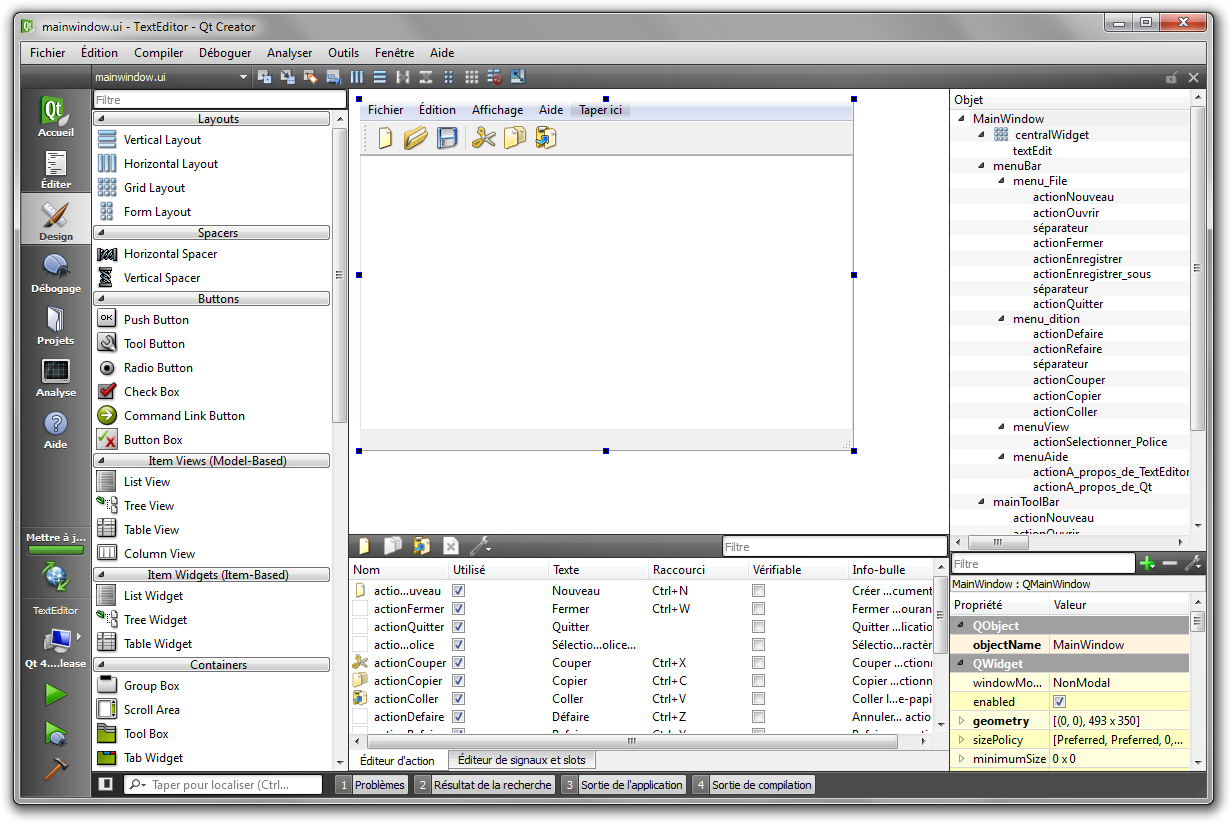
\includegraphics[scale=0.3]{Qt_creator.png}
            \end{center}

            \caption{Éditeur d'interface WYSIWYG de Qt Creator}
            \label{Qt Creator}
        \end{figure}

    \newpage

    \section{Gestionnaire de version et travail collaboratif Git}
        \paragraph{}
            Bien que n'étant qu'en binôme, travailler en équipe sur un même code sans outil approprié se révèle souvent être un enfer. En effet, la modification d'un fichier peut entrainer des incompatibilités et des bugs dans le reste du programme. Et c'est à ce genre de problèmes que vient répondre un gestionnaire de version.
            \\ Tout comme les frameworks graphiques, il existe plusieurs solutions sur le marché, on retiendra essentiellement svn et git. Le choix de git fût immédiat car maitrisé par l'ensemble de l'équipe. 
            \\ Git a été créé en 2005 par Linus Torvalds, créateur de noyau linux, devant la nécessité de cannaliser et organiser les contributions des milliers de contributeurs de linux. C'est le gestionnaire de version le plus utilisé, et est un réel standard dans le monde du développement logiciel.

        \paragraph{}
            Git est un outil déscentralisé, un service : il doit être herbergé par un serveur. Là ou il est possible d'être indépendant et d'héberger son propre serveur github, nous avons préferé nous rabattre sur un hébergeur gratuit et public, github.
            \\ Ce choix est motivé et par la facilité d'utilisation qu'offre github, mais aussi par la volonté d'avoir un programme libre. Github met ainsi à 
            disposition librement et pour tous notre programme, sous la licence de notre choix (ici MIT).
            
            \begin{figure}[h]
                \begin{center}
                    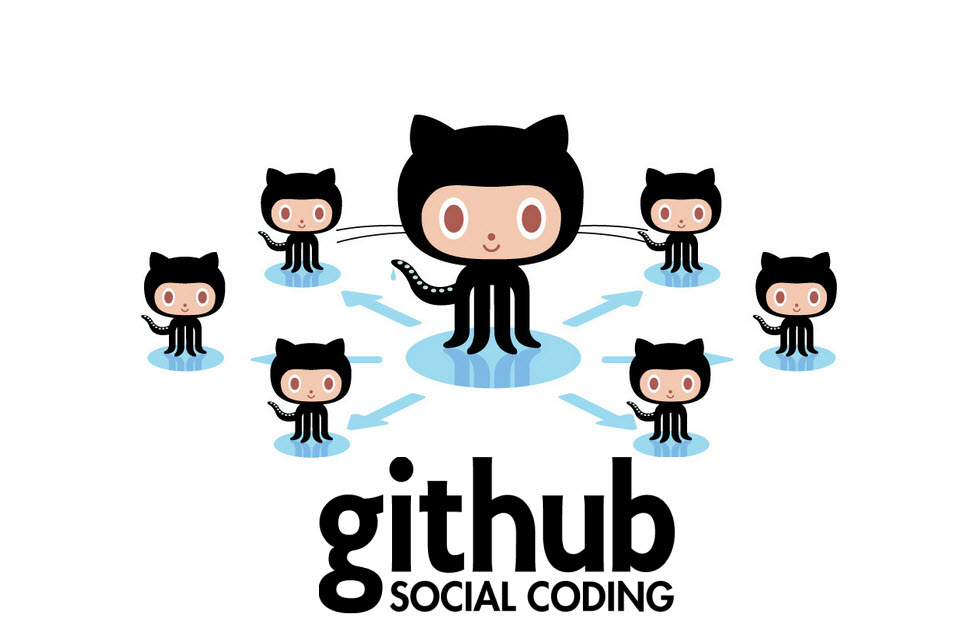
\includegraphics[scale=0.3]{logo_github.jpg}
                \end{center}

                \caption{Logo de github}
                \label{github}
            \end{figure}

    \newpage

    \section{Générateur de documentation Doxygen}
        